\documentclass{article}
\usepackage{braket,amsmath,graphicx,color,caption}
\usepackage[hidelinks]{hyperref}
\usepackage[margin=0.5in]{geometry}
\begin{document}
\title{\bf R. Shankar's RG derivation for Landau Fermi liquid and BCS instability}
\author{Abhirup Mukherjee}
\maketitle

\begin{abstract}
This is an expansion of R. Shankar's derivation (Shankar, 1993) of the Landau Fermi liquid effective Hamiltonian and its possible BCS instability by applying the renormalization group technique on a general 2D interacting fermionic system with a circular Fermi surface. I have added a short introduction to the philosophy of renormalisation group. Certain non-trivial arguments and calculations have also been fleshed out. Where possible, certain parts have been simplified.
\end{abstract}

\section{Short primer on the renormalization group}
The philosophy of the renormalization group approach is to integrate out high energy modes from a microscopic Hamiltonian and observe how the couplings morph in the process. This allows us to write down a low-energy effective Hamiltonian for the problem which can be used to describe low-energy excitations as well as universal features which depend on the short-distance details only through a small number of couplings which are, as a result, termed to be \textit{relevant}.

Say we have a free energy \(\mathcal{F}\), characterized by a scalar field \(\phi\). The partition function can be written as a path integral over all configurations of \(\phi_k\):
\begin{equation}\begin{aligned}
\label{oldpart}
Z = \int \mathcal{D}\phi \;\exp\left\{-\mathcal{F}(\phi)\right\}
\end{aligned}\end{equation}
where 
\begin{equation}\begin{aligned}
\mathcal{F}[\phi] = \int_0^\Lambda dk \;f[\phi(k)]
\end{aligned}\end{equation}
Let us assume there is a natural momentum cutoff in the problem \(\Lambda\). There are three distinct steps involved in the RG procedure:
\begin{itemize}
	\item Integrate out modes in the range \(\left[b\Lambda,\Lambda\right]\), where \(b < 1\).
	\item Rescale the momenta to keep the limits unchanged so that we can compare the new partition function with the previous one: \(k^\prime = \frac{k}{b}\)
	\item Rescale the fields so as to keep at least one term in the partition function unchanged (usually the Gaussian term) so that we can compare the changes in the rest of the terms: \(\phi^\prime = \lambda\phi\)
\end{itemize}

In a single iteration of the RG, the first step is to reduce the cutoff to \(b\Lambda\), \(b\) obviously being less than 1. To facilitate this, we separate the fields into high momentum and low momentum parts:
\begin{equation}\begin{aligned}
\phi(k) = \phi^<(k) + \phi^>(k)
\end{aligned}\end{equation}
where \(\phi^>\) is nonzero only for \(k>b\Lambda\) and \(\phi^<\) is nonzero in the remaining region.
\begin{equation}\begin{aligned}
\phi^>(k) = \begin{cases} \phi(k), &b\Lambda < k <\Lambda\\ 0 &\text{otherwise} \end{cases},\\
\phi^<(k) = \begin{cases} 0, &b\Lambda < k <\Lambda\\ \phi(k), &\text{otherwise} \end{cases}
\end{aligned}\end{equation}
This allows us to write the free energy in the following form:
\begin{equation}\begin{aligned}
\mathcal{F}[\phi(k)] = \mathcal{F}^<[\phi^<] + \mathcal{F}^>[\phi^>] + \mathcal{F}^i[\phi^>,\phi^<]
\end{aligned}\end{equation}
We can now integrate the high momentum modes:
\begin{equation}\begin{aligned}
	Z &= \int \mathcal{D}\phi^<\; \exp\left\{\mathcal{F}^<[\phi^<]\right\}\int \mathcal{D}\phi^>\;\exp\left\{\mathcal{F}^>[\phi^>] + \mathcal{F}^i[\phi^>,\phi^<]\right\}\\
	  &=\int \mathcal{D}\phi^<\; Z^>[\phi^<]\exp\left\{\mathcal{F}^<[\phi^<]\right\}
\end{aligned}\end{equation}
We can now define the remaining integrand as a new effective free energy \(\mathcal{F}_b\):
\begin{equation}\begin{aligned}
	Z  =\int \mathcal{D}\phi^<\; \exp\left\{\mathcal{F}_b[\phi^<]\right\}
\end{aligned}\end{equation}
where
\begin{equation}\begin{aligned}
\mathcal{F}_b[\phi^<] = \int_0^{b\Lambda} dk\;{f_b}[\phi(k)]
\end{aligned}\end{equation}
Our goal is to compare this partition function with the one in eq.~\ref{oldpart}. In order to do this, however, we need to make sure the integral is over the same limits in both cases. The old partition function integrates over all \(\phi\), while the new one integrates only up to \(b\Lambda\). To remedy this, we define new momenta by re-scaling the old momenta, \(k^\prime = \frac{k}{b}\). This will take the limit of integration back to \(\Lambda\):
\begin{gather}
\mathcal{F}_b[\phi^<] = \int_0^{b\Lambda} dk\;{f_b}[\phi(k)] = \int_0^{\Lambda} dk^\prime\;{f_b}[\phi(k^\prime)]\\
Z = \int \mathcal{D}\phi\;\exp\left\{\mathcal{F}_b[\phi]\right\}
\end{gather}
There is one final thing to do. Since an overall scalar factor in the free energy does not make any difference, we would like to make this explcit by fixing the prefactor of one of the terms in the free energy functional. This involves scaling the fields \(\phi\):
\begin{equation}\begin{aligned}
\phi^\prime = \lambda \phi
\end{aligned}\end{equation}
With this transformation, the final partition function is
\begin{equation}\begin{aligned}
	Z = \int \mathcal{D}\phi^\prime\;\exp\left\{\mathcal{F}_b[\phi^\prime]\right\}
\end{aligned}\end{equation}
We can now compare the free energies \(\mathcal{F}(\phi)\) and \(\mathcal{F}_b(\phi^\prime)\). This will lead to scaling equations for the couplings that make up the free energy.
\section{Setting up the problem of interacting fermions}
The problem we are trying to solve is that of interacting Fermions placed in the two-dimensional continuum. The Fermi surface will be spherical. The Hamiltonian for  the non-interacting system is very simple:
\begin{equation}\begin{aligned}
\mathcal{H} = \int d\mathbf{K}\; E(\mathbf{K})\hat n(\mathbf{K})
\end{aligned}\end{equation}
where \(E\) is the single particle dispersion, \(\mathbf K\) is the momentum and \(\hat n = \psi^\dagger \psi\) is the number operator. Our goal is to determine what happens when we bring interactions into the problem. The action for the non-interacting case is determined by calculating the partition function. The partition function turns out to be
\begin{equation}\begin{aligned}
	Z = \int \mathcal{D}\psi^\dagger \mathcal{D}\psi\exp\left\{\int d\tau\;d\mathbf{K}\;\psi_\mathbf{K,\sigma}^\dagger\left(\frac{\partial}{\partial \tau} - E_\mathbf{K,\sigma} \right)\psi_\mathbf{K,\sigma}\right\}
\end{aligned}\end{equation}
Using the Fourier transform
\begin{equation}\begin{aligned}
\psi(\tau) = \int d\omega e^{i\omega \tau}\psi(\omega)~,
\end{aligned}\end{equation}
the action can be expressed as an integral over the energy \(\omega\).
\begin{equation}\begin{aligned}
	S_0 &= \int d\tau\;d\mathbf{K}\;\int d\omega e^{-i\omega \tau}\psi_\mathbf{K,\sigma}^\dagger(\omega)\left(\frac{\partial}{\partial \tau} - E_\mathbf{K,\sigma} \right)\int d\omega^\prime e^{i\omega^\prime \tau}\psi_\mathbf{K,\sigma}(\omega^\prime)\\
	    &= \int d\mathbf{K}\;\int d\omega d\omega^\prime \psi_\mathbf{K,\sigma}^\dagger(\omega)\left(i\omega^\prime - E_\mathbf{K,\sigma} \right) \psi_\mathbf{K,\sigma}(\omega^\prime)\int d\tau e^{i\left(\omega^\prime - \omega\right)\tau}\\
	    &= \int d\omega\;d\mathbf{K}\; \psi_{\mathbf K,\sigma}^\dagger \left(i\omega - E_{\mathbf{K},\sigma}\right)\psi_{\mathbf{K},\sigma}
\end{aligned}\end{equation}

\begin{minipage}{0.55\textwidth}
We now modify the setup to suit the problem better. The Pauli exclusion principle ensures that all states up to the Fermi momentum \(\mathbf{k}_F\) are filled, in the ground state. Excitations, then, involve adding Fermions above the Fermi momentum and deleting electrons below the Fermi momentum. To this end, we can define an electron at the Fermi energy \(E_F\) to have zero energy and measure the energy of excitations from the Fermi surface: \(\xi_{\mathbf K} = E_{\mathbf K} - E_F\).
We can now specify the cutoff: The only excitations we will be considering are those that are within a radial distance \(\Lambda\) from the Fermi surface \(\mathbf{k}_F\). Since the Fermi surface itself is spherical, it is easier if we split the momentum vector into a radial and an angular component:
\begin{equation}\begin{aligned}
\int d\mathbf{K} = \int_0^{2\pi} d\theta \int_0^\infty dK
\end{aligned}\end{equation}
The radial component is, by definition, positive. \(\theta\) as a result goes from \(0\) to \(2\pi\). The cutoff implies that we will only consider \(K \in \left[k_F - \Lambda, k_F + \Lambda\right]\).
\begin{equation}\begin{aligned}
	S_0 = \int_{-\infty}^\infty d\omega\;\int_0^{2\pi} d\theta \int_{k_F - \Lambda}^{k_F + \Lambda}  dk\; \psi_{\mathbf{K},\sigma}^\dagger \left(i\omega - \xi_{\mathbf{K}}\right)\psi_{\mathbf{K},\sigma}
\end{aligned}\end{equation}
Since we are only interested in excitations close to the Fermi surface, we can approximate the single particle energy as
\begin{equation}\begin{aligned}
	\xi_\mathbf{K} = \frac{\hbar^2}{2m}\left(K^2 - k_F^2\right) = \frac{\hbar^2}{2m}\left(K - k_F\right)\left(K + k_F\right) \\
	\approx \frac{\hbar^2}{2m}\left(K - k_F\right)2k_F = \hbar \left(K-k_F\right)v_F
\end{aligned}\end{equation}
Choosing units such that \(v_F = \hbar = 1\), we get
\begin{equation}\begin{aligned}
	\xi_\mathbf{K} \equiv E_\mathbf{K} - E_F = K - k_F
\end{aligned}\end{equation}
Since we see that \(k_F\) is popping up everywhere, we might as well define \(k = K - k_F\). This will reduce each of the limits by \(k_F\):
\begin{gather}
	\xi_\mathbf{K} = k \\
	S_0 = \int_{-\infty}^\infty d\omega\;\int_0^{2\pi} d\theta \int_{- \Lambda}^{\Lambda}  dk\; \psi_{\mathbf{K},\sigma}^\dagger \psi_{\mathbf{K},\sigma}\label{action}
\end{gather}
\end{minipage}
\hspace*{\fill}
\begin{minipage}{0.4\textwidth}
\centering
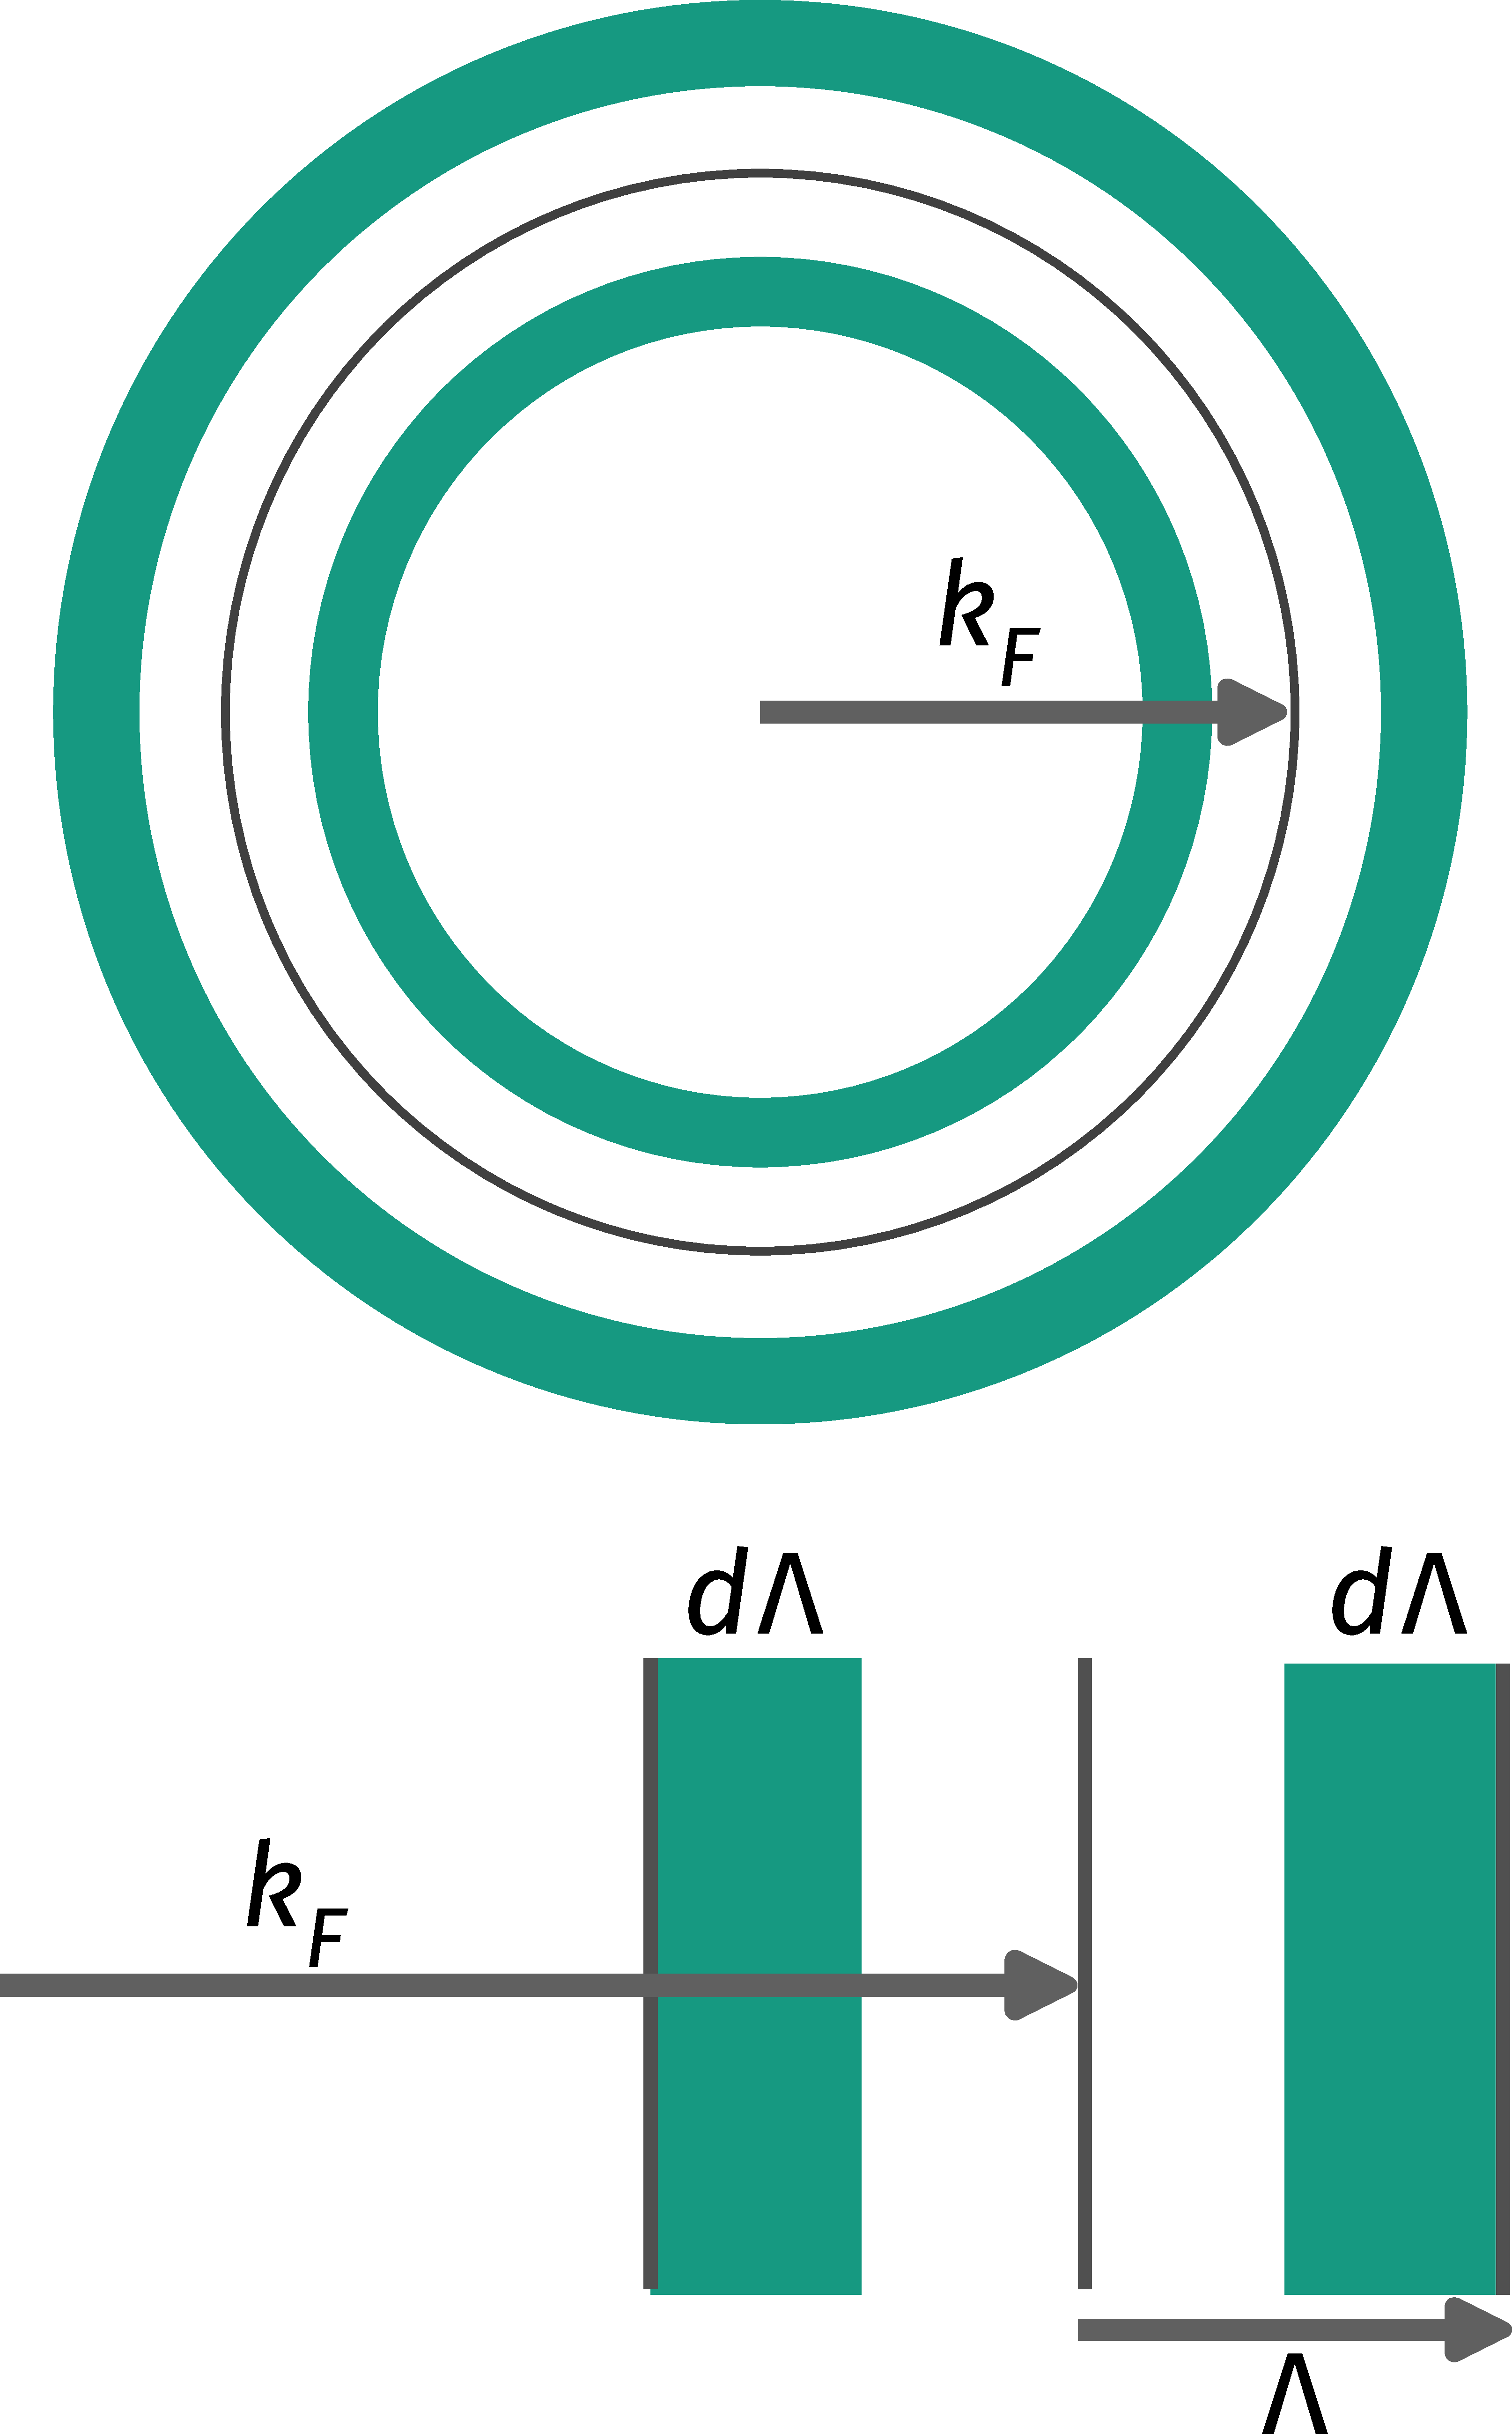
\includegraphics[width=0.8\textwidth]{./figures/fermi-rg.pdf}
\captionof{figure}{Left: The intermediate dotted circle represents the Fermi surface, while the inner and outer dotted circles represent the lower and upper cutoffs at \(k_F \pm \Lambda\). We are concerned with the momentum space region in between the inner and outer dotted circles. Right: Zoom in of a particular direction of the momentum space. The yellow region represents the region of momentum space that will be integrated over, in each RG step. It extends up to \(d\Lambda\) from the cutoff \(\Lambda\).} 
\end{minipage}

\section{Noninteracting fixed point}
As mentioned in the previous section, the first step involves reducing the cutoff and integrating out the fast modes. Let the reduced cutoff be \(b\Lambda\), \(b<1\). We can split the action into high momentum and low momentum part:
\begin{equation}\begin{aligned}
	S_0^< &= \int_{-\infty}^\infty d\omega\;\int_0^{2\pi} d\theta \int_{- b\Lambda}^{b\Lambda}dk~\psi_{\mathbf{K},\sigma}^\dagger \left(i\omega - k\right)\psi_{\mathbf{K},\sigma}\\
	S_0^> &= \int_{-\infty}^\infty d\omega\;\int_0^{2\pi} d\theta \int_{\left[-\Lambda,- b\Lambda\right]}^{\left[b\Lambda,\Lambda\right]}dk~\psi_{\mathbf{K},\sigma}^\dagger \left(i\omega - k\right)\psi_{\mathbf{K},\sigma}
\end{aligned}\end{equation}
Then,
\begin{equation}\begin{aligned}
	Z = \int \prod_{k<b\Lambda} d\psi^\dagger_{\mathbf{K},\sigma} d\psi_{\mathbf{K},\sigma} e^{S_0^<}\int \prod_{k>b\Lambda} d\psi^\dagger_{\mathbf{K},\sigma} d\psi_{\mathbf{K},\sigma} e^{S_0^>}
\end{aligned}\end{equation}
Since the modes are decoupled, the result of the high momentum integral does not depend on the low momentum operators; as a result, we can drop that factor that results from the integration. The next step involves rescaling the momenta and energy to recover the original limit. This means we should define new momenta and energy \(k^\prime, \omega^\prime\):
\begin{gather}
k^\prime = \frac{1}{b}k~,\\
\omega^\prime = \frac{1}{b}\omega~.
\end{gather}
This will modify the action as
\begin{equation}\begin{aligned}
	S_0^< &= \int_{-\infty}^\infty b d\omega^\prime\;\int_0^{2\pi} d\theta \int_{-\Lambda}^{\Lambda}b dk^\prime\psi_{\mathbf{K},\sigma}^\dagger \left(ib\omega^\prime - bk^\prime\right)\psi_{\mathbf{K},\sigma}\\
	      &=\int_{-\infty}^\infty d\omega^\prime\;\int_0^{2\pi} d\theta \int_{-\Lambda}^{\Lambda}dk^\prime\psi_{\mathbf{K},\sigma}^\dagger b^{3} \left(i\omega^\prime - k^\prime\right)\psi_{\mathbf{K},\sigma}
\end{aligned}\end{equation}
Since we are only scaling the radial distance, \(\theta\) will not scale. If we want to compare this new action with the old action eq.~\ref{action}, we need to rescale the fields \(\psi,\psi^\dagger\) to get rid of any global factors. This was the third step mentioned in the previous section. Its obvious that the following rescaling takes care of the \(b^3\) factor: \(\psi^\prime_{\mathbf{K}^\prime} = b^{\frac{3}{2}}\psi_\mathbf{K}\). The final partition function for the reduced cutoff is
\begin{equation}\begin{aligned}
	Z^< = \int \mathcal{D}{\psi^\prime}^\dagger \mathcal{D}{\psi^\prime}\exp\left\{\int_{-\infty}^\infty d\omega^\prime\;\int_0^{2\pi} d\theta \int_{-\Lambda}^{\Lambda}dk^\prime\psi_{\mathbf K^\prime,\sigma}^\dagger \left(i\omega^\prime - k^\prime\right)\psi_{\mathbf K^\prime,\sigma}\right\}
\end{aligned}\end{equation}
\textbf{This is identical to the partition function we started with. This means that the noninteracting theory is an RG fixed point.}
\section{Quadratic interaction: tree-level RG}
\begin{minipage}{0.55\textwidth}
We now introduce quadratic interactions through scattering via a potential \(u(k,\omega)\). Owing to momentum conservation, such a term must have the form
\begin{equation}\begin{aligned}
	\int_{-\infty}^\infty d\omega\;\int_0^{2\pi} d\theta \int_{-\Lambda}^{\Lambda}dk \;u(K,\omega)\psi_{\mathbf{K},\sigma}^\dagger\psi_{\mathbf{K},\sigma}
\end{aligned}\end{equation}
\end{minipage}
\hspace*{\fill}
\begin{minipage}{0.3\textwidth}
	\centering
	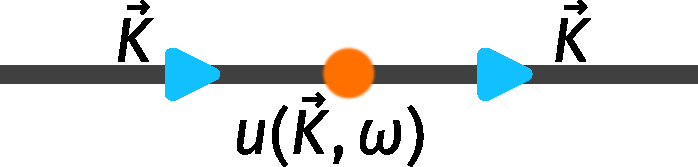
\includegraphics[width=0.9\textwidth]{./figures/tree_quadratic.pdf}
	\captionof{figure}{Momentum-conserving quadratic interaction at tree-level}
\end{minipage}

Such a term is diagonal in the momentum and we can again carry out the three re-scaling operations mentioned previously:
\begin{gather}
	k^\prime = b^{-1} k\\
	\omega^\prime = b^{-1} \omega\\
{\psi^\prime}^\dagger_\mathbf{k^\prime,\sigma}{\psi^\prime}_\mathbf{k^\prime,\sigma} = b^{3}\psi^\dagger_\mathbf{k,\sigma}\psi_\mathbf{k,\sigma}
\end{gather}
The interaction term then changes to
\begin{equation}\begin{aligned}
	\int_{-\infty}^\infty d\omega^\prime\;\int_0^{2\pi} d\theta \int_{-\Lambda}^{\Lambda}dk^\prime ~ b^{-1} ~ u(K^\prime,\omega^\prime){\psi^\prime}_{\mathbf{K},\sigma}^\dagger\psi_{\mathbf{K},\sigma}
\end{aligned}\end{equation}
We thus see that, as a result of decreasing the cutoff, the interaction potential renormalizes as
\begin{equation}\begin{aligned}
	u(K,\omega) \to b^{-1} u(K^\prime,\omega^\prime)
\end{aligned}\end{equation}
To determine the effect of this, we expand \(u\) in a Taylor series around \(\mathbf{k}=0,\omega=0\):
\begin{equation}\begin{aligned}
	u(K,\omega) &= u_{00} + \omega u_{10} + k u_{01} + \omega^2 u_{20} + k^2 u_{02} + k\omega u_{11} + ...\\
	\to b^{-1}u(K^\prime,\omega^\prime) &= b^{-1}u_{00} + b^{-1} b\left(\omega^\prime u_{10} + k^\prime u_{01}\right) + b^{-1} b^{2} \left({\omega^\prime}^2 u_{20} + {k^\prime}^2 u_{02} + \omega^\prime k^\prime u_{11}\right) + ...\\
						   &= b^{-1}u_{00} + \omega^\prime u_{10} + k^\prime u_{01} + b \left({\omega^\prime}^2 u_{20} + {k^\prime}^2 u_{02} + \omega^\prime k^\prime u_{11}\right)...
\end{aligned}\end{equation}
where \(u_{mn} = \left(\partial^m_\omega \partial^n_k u\right)_{\omega \to 0, k \to 0}\). The various terms scale as follows:
\begin{equation}\begin{aligned}
	u_{mn} \to u_{mn}^\prime = b^{m + n - 1}u_{mn}, ~b<1
\end{aligned}\end{equation}
The zeroth order term is relevant - it increases as we scale down to low energies. The first order terms are marginal - they do not change, at least at tree level. Higher terms are irrelevant - they decay upon renormalization.

Even though the zeroth order term is relevant,  such a term already exists in the non-interacting action - the chemical potential term. Since the energies scale as \(\omega^\prime = b\omega\), the chemical potential will also scale as \(\mu^\prime = b \mu\). Hence, we can absorb the relevant zeroth order part of the quadratic fluctuation into the chemical potential:
\begin{gather}
	\mu_\text{eff} = \mu + u_{00} = b \mu^\prime + bu^\prime_{00} = b \mu_\text{eff}^\prime
\end{gather}

The marginal first order terms are also present in the non-interacting action, and hence can again be absorbed into those terms. The conclusion is therefore that adding quadratic interactions do not destroy the non-interacting action, it simply renormalizes certain terms of the non-interacting action.
\section{Quartic interaction: tree-level RG}
Next we consider quartic interactions. Translational invariance and time-reversal symmetry requires such scattering events to conserve total momentum and spin:
\begin{equation}\begin{aligned}
	\int V(1,2,3,4)\psi_{4,\sigma}^\dagger\psi_{2,\sigma^\prime}\psi_{3,\sigma}^\dagger\psi_{1\sigma^\prime} \delta(\mathbf{K_4}+\mathbf{K_3} - \mathbf{K_2} - \mathbf{K_1})\delta({\omega_4}+{\omega_3} - {\omega_2} - {\omega_1})
\end{aligned}\end{equation}
\begin{minipage}{0.6\textwidth}
where \(\int\) stands for  \(\prod_{i=1}^4\int_{-\infty}^\infty d\omega_i \int_{0}^{2\pi}d\theta_i \int_{-\Lambda}^\Lambda dk_i~\). There are now four sets of variables instead of just one: \(\{(\omega_i, \mathbf{K_i}) : i=[1,4]\}\). \(V(1,2,3,4) = V(\{\omega_i, \mathbf{K_i}\})\) is the scattering potential and in general depends on all the momenta and energies. The delta functions conserve total momentum and total energy. Here, \(d\omega\) stands for \(d\omega_1d\omega_2d\omega_3d\omega_4\) and \(dk\) stands for \(dk_1dk_2dk_3dk_4\). The fields \(\psi_{i\sigma} = \psi_{\mathbf{K_i}\sigma}\) of course depend on the momenta and energies. 

We will now try to eliminate one set of variables, say the fourth set \((\omega_4, \mathbf{K_4})\). We can easily integrate over \(\omega_4\) by consuming the energy \(\delta\)-function. Since all the \(\omega_i\) integrals are independent, the condition inside the \(\delta\)-function does not constrain the values of the remaining \(\omega_i\).
\end{minipage}
\hspace*{\fill}
\begin{minipage}{0.3\textwidth}
\begin{center}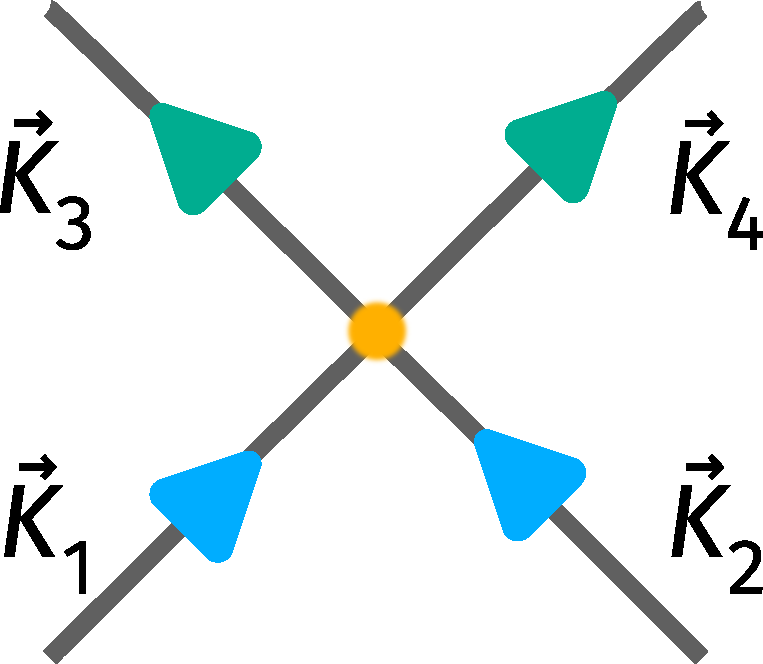
\includegraphics[width=0.7\textwidth]{./figures/term.pdf}\end{center}
\captionof{figure}{Tree-level four-Fermion scattering}
\end{minipage}

The result of this integration is
\begin{equation}\begin{aligned}
	\int_{-\infty}^\infty d\omega_1 d\omega_2 d\omega_3\;\int_0^{2\pi} \prod_{i=1}^4 d \theta_i \int_{-\Lambda}^{\Lambda}\prod_{i=1}^4 dk_i \;V\psi_{4,\sigma}^\dagger\psi_{2,\sigma^\prime}\psi_{3,\sigma}^\dagger\psi_{1\sigma^\prime} \delta(\mathbf{K_4}+\mathbf{K_3} - \mathbf{K_2} - \mathbf{K_1})
\end{aligned}\end{equation}
The fields and \(V\) now depend only on the remaining frequencies \(\omega_1,\omega_2\) and \(\omega_3\). We now need to tackle the other \(\delta\)-function with the goal of integrating \(\mathbf{K_4}\). The situation is different from the \(\omega_i\) integral because the momenta have an additional constraint: they must lie within the annulus \(\left[-\Lambda,\Lambda\right]\). Merely replacing the \(\mathbf{K_4}\) integral with the substitution \(\mathbf{K_4} = \mathbf{K_3} - (\mathbf{K_2} + \mathbf{K_1})\) (what we did for \(\omega_4\)) will not work, because there are combinations of the other three momenta that will then take \(\mathbf{K_4}\) outside the annulus. One example is the following combination:
\begin{equation}\begin{aligned}
	\mathbf{K_1} = -k_F \hat x,~\mathbf{K_2} = \left(-\Lambda + k_F\right)\hat x,~\mathbf{K_3} = \left( \Lambda + k_F \right) \hat x~\implies |\mathbf{K_4}| = 2\Lambda + k_F~.
\end{aligned}\end{equation}
To prevent this, will carry out the integration without any constraint but then multiple the result with \(\theta(\Lambda - |k_4|)\) to impose the constraint, where \(k_4 = |\mathbf{K_3} - (\mathbf{K_2} + \mathbf{K_1})| - k_F\):
\begin{equation}\begin{aligned}
	\prod_{i=1}^3\int_{-\infty}^\infty d\omega_i\;\int_0^{2\pi} d\theta_i \int_{-\Lambda}^{\Lambda}dk_i \;V(1,2,3)\psi_{4,\sigma}^\dagger\psi_{2,\sigma^\prime}\psi_{3,\sigma}^\dagger\psi_{1\sigma^\prime}\theta(\Lambda - |k_4|)~.
\end{aligned}\end{equation}
\(\psi_{4}\) depends on \(\mathbf{K_3} - (\mathbf{K_2} + \mathbf{K_1})\). The Heaviside function restricts \(\mathbf{K_4}\) to the proper range.

We need to check how this Heaviside function \(\theta(\Lambda - |k_4|) = \theta(\Lambda - ||\mathbf{K_3} - \mathbf{K_2} - \mathbf{K_1}| - k_F|) \) changes under the scaling. The relevant steps are decreasing the cutoff to \(b\Lambda\) and increasing all momenta \(k_i\) to \(k_i/b\). \(k_4\) scales as:
\begin{equation}\begin{aligned}
	k_4 &= |\mathbf{K_3} - \mathbf{K_2} - \mathbf{K_1}| - k_F\\
	    &= |\left(k_F + k_3\right)\hat K_3 - \left(k_F + k_2\right)\hat K_2 - \left(k_F + k_1\right)\hat K_1| - k_F\\
	    &= |\left(k_F + b k^\prime_3\right)\hat K_3 - \left(k_F + b k^\prime_2\right)\hat K_2 - \left(k_F + b k^\prime_1\right)\hat K_1| - k_F\\
	    &= b\left|\left(\frac{1}{b}k_F + k^\prime_3\right)\hat K_3 - \left(\frac{1}{b}k_F + k^\prime_2\right)\hat K_2 - \left(\frac{1}{b}k_F + k^\prime_1\right)\hat K_1\right| - \frac{1}{b}k_F\\
	    &= b~k_4^\prime(\mathbf{K_i^\prime}, \frac{k_F}{b})\\
\end{aligned}\end{equation}
The Heaviside function therefore scales as
\begin{equation}\begin{aligned}
	\theta(\Lambda - |k_4|) \to \theta(b\Lambda - b|k_4^\prime|) = \theta\left(\Lambda - \left|k_4^\prime\left(\mathbf{K_i^\prime},\frac{k_F}{b}\right)\right|\right)
\end{aligned}\end{equation}
The final step of rescaling the fields does not affect the Heaviside function in any way. We thus see that the Heaviside function does not return to its original form; \(k_F\) has to go to \(k_F/b\). In order to remedy this, we replace the Heaviside function by an exponential decay:
\begin{equation}\begin{aligned}
	\exp\left\{-\frac{|k_4|}{\Lambda}\right\}
\end{aligned}\end{equation}
The effect of this exponential decay is similar to the Heaviside function; it suppresses the effect of the \(k_4\) that lie outside the allowed region,  \(|k_4| > \Lambda\). In the limit of approaching the Fermi surface \((\Lambda \rightarrow 0)\), the exponential takes the form of the Heaviside function:
\begin{equation}\begin{aligned}
	\lim_{\Lambda \to 0} \exp\left\{-\frac{|k_4|}{\Lambda}\right\} = \begin{cases} 1, &\text{ when } |k_4|<\Lambda \\ 0, &\text{ when } |k_4|>\Lambda \end{cases} = \theta(\Lambda - |k_4|)
\end{aligned}\end{equation}
The quartic term takes the form
\begin{equation}\begin{aligned}
	\prod_{i=1}^3\int_{-\infty}^\infty d\omega_i\;\int_0^{2\pi} d\theta_i \int_{-\Lambda}^{\Lambda}dk_i \;V(1,2,3)\psi_{4,\sigma}^\dagger\psi_{2,\sigma^\prime}\psi_{3,\sigma}^\dagger\psi_{1\sigma^\prime}\exp\left\{-\frac{|k_4|}{\Lambda}\right\}
\end{aligned}\end{equation}
To see how this exponential factor scales with the renormalization, note that
\begin{equation}\begin{aligned}
\label{k4}
k_4 &= \left|\mathbf{K_3} - \mathbf{K_2} - \mathbf{K_1}\right| - k_F \\
    &= \left|\left(k_3 + k_F\right)\hat K_3 - \left(k_2 + k_F\right)\hat K_2 - \left(k_1 + k_F\right)\hat K_1\right| - k_F\\
    &=\left|k_F\left(\hat K_3 - \hat K_2 - \hat K_1\right) + \left(\mathbf{k_3} - \mathbf{k_2} - \mathbf{k_1}\right)\right| - k_F
\end{aligned}\end{equation}
The second term, \(\mathbf{k_3} - \mathbf{k_2} - \mathbf{k_1}\), is of order at most \(\Lambda\), because that is the highest value \(k_4\) can take:
\begin{equation}\begin{aligned}
	(k_4)_\mathrm{max} &= k_F + |\mathbf{k_3} - \mathbf{k_2} - \mathbf{k_1}|_\mathrm{max} - k_F = |\mathbf{k_3} - \mathbf{k_2} - \mathbf{k_1}|_\mathrm{max}\\
	\implies |\mathbf{k_3} - \mathbf{k_2} - \mathbf{k_1}|_\mathrm{max} &= (k_4)_\mathrm{max} = \Lambda
\end{aligned}\end{equation}
The only situation in which this second term can be comparable to the first term is when both are of order \(\Lambda\), but for such values, \(|k_4|\) will be of the order of \(k_F\):
\begin{equation}\begin{aligned}
	|k_4| \sim |2\Lambda - k_F| \sim |k_4|
\end{aligned}\end{equation}
Such cases will be suppressed by the exponential factor. Therefore, we can ignore such cases, and assume that the second term in eq.~\ref{k4} can always be neglected when compared to the first:
\begin{equation}\begin{aligned}
	k_4 \approx k_F\left|\hat K_3 - \hat K_2 - \hat K_1\right| - k_F
\end{aligned}\end{equation}
Under the renormalization, the unit vectors will not scale because they are simply directions on the Fermi surface and are dimensionless. Therefore,
\begin{equation}\begin{aligned}
	\exp\left\{-\frac{\left|k_F\left|\hat K_3 - \hat K_2 - \hat K_1\right| - k_F\right|}{\Lambda}\right\}&\rightarrow\exp\left\{-\frac{\left|k_F\left|\hat K_3 - \hat K_2 - \hat K_1\right| - k_F\right|}{b\Lambda}\right\}\\
															 &=\exp\left\{-\frac{\left|k_F\left|\hat K_3 - \hat K_2 - \hat K_1\right| - k_F\right|}{\Lambda}\left(1 + \frac{b-1}{b}\right)\right\}\\
	\implies \exp\left\{-\frac{|k_4|}{\Lambda}\right\} &\rightarrow \exp\left\{-\frac{|k_4|}{\Lambda}\right\}\exp\left\{\left(1 - \frac{1}{b}\right)\frac{|k_4|}{\Lambda}\right\}
\end{aligned}\end{equation}
Therefore, under the renormalization, the exponential gets multiplied by a factor
\begin{equation}\begin{aligned}
	\exp\left\{\left(1 - \frac{1}{b}\right)\frac{|k_4|}{\Lambda}\right\}
\end{aligned}\end{equation}
As \(\Lambda \rightarrow 0^+\), the argument of the exponential will go to \(-\infty\) and the factor will vanish, provided \(|k_4| \neq 0\). 
\\\\
\begin{minipage}{0.6\textwidth}
The only terms that will survive are those for which \(|k_4|\) vanishes:
\begin{gather}
	|k_4| \approx k_F\left(\left|\hat K_3 - \hat K_2 - \hat K_1\right| - 1\right)=0\\
	\implies \left(\hat K_3 - \hat K_2 - \hat K_1\right)^2 = 1\label{eqtn}
\end{gather}
The only choices of momenta that will survive are the ones in the directions that satisfy the above equation. To find the possible angles for that equation, let \(\hat x \equiv \hat K_3\) and \(\hat K_{1,2} = \cos \theta_{1,2}\hat x + \sin\theta_{1,2}\hat y\). As defined, \(\theta_1\) is the angle between \(\hat K_1\) and \(\hat K_3\), and \(\theta_2\) is that between \(\hat K_2\) and \(\hat K_3\). 
\end{minipage}
\hspace*{\fill}
\begin{minipage}{0.35\textwidth}
	\centering
	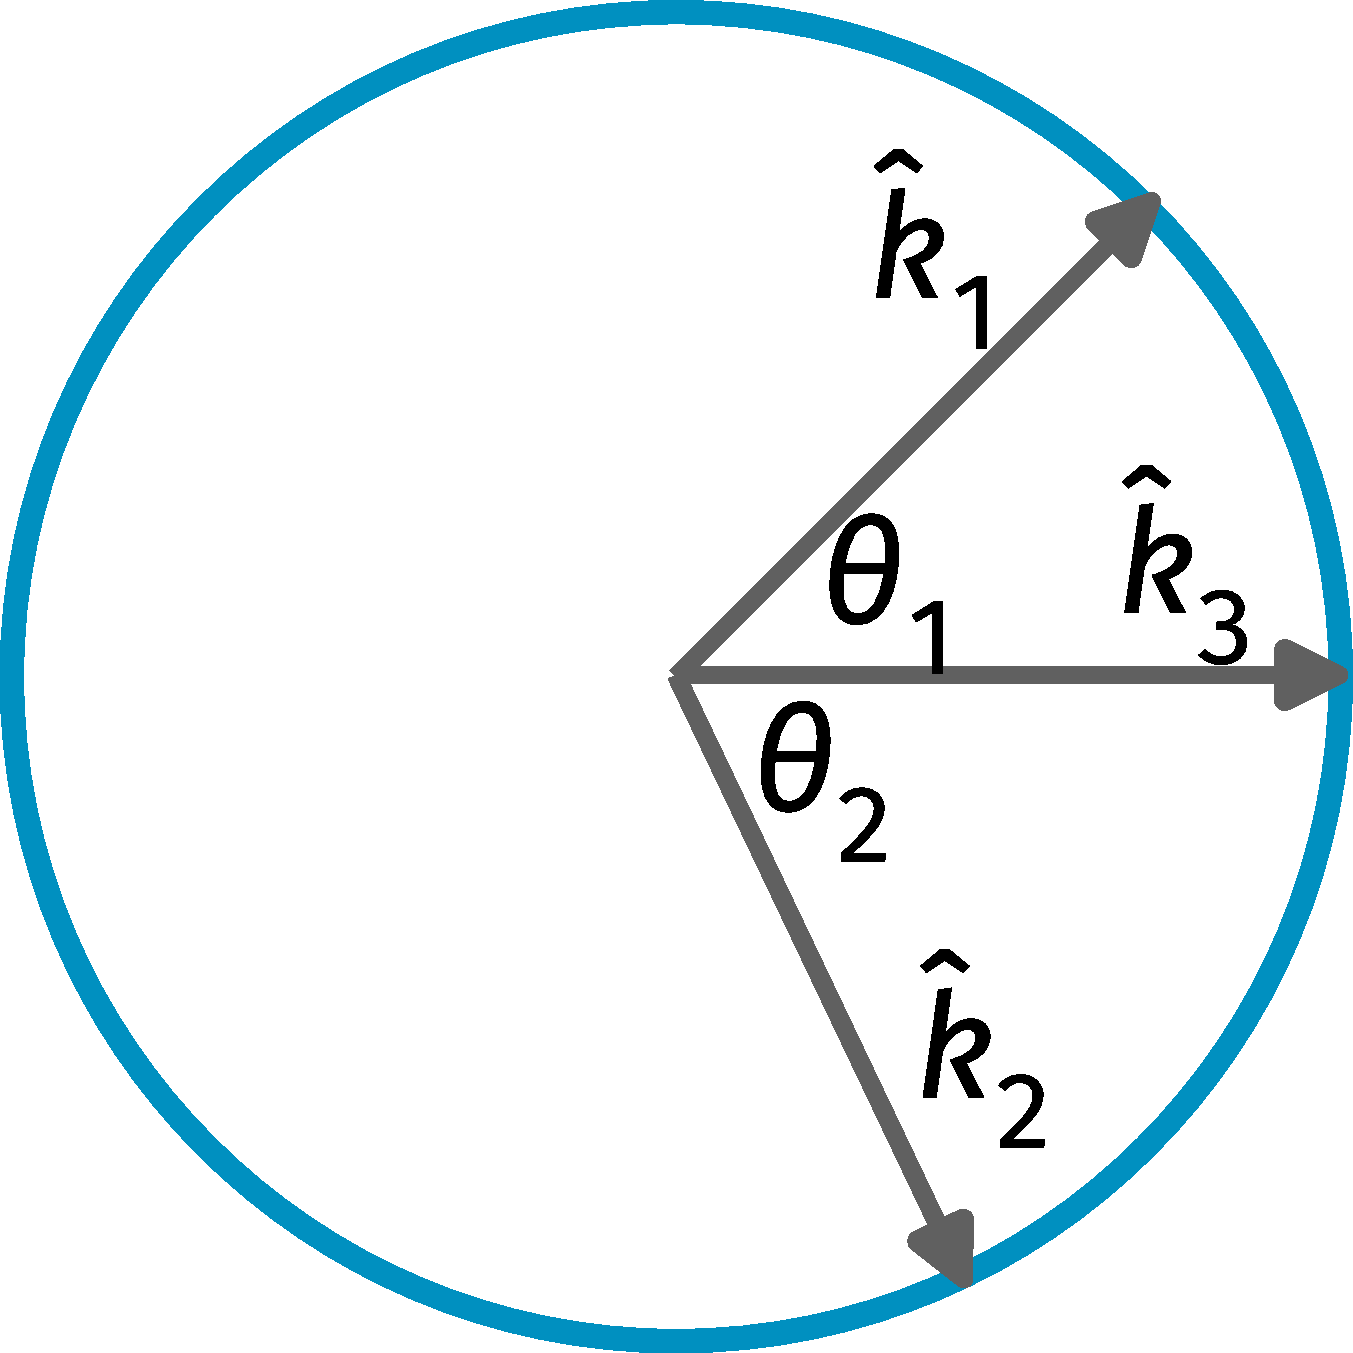
\includegraphics[width=0.65\textwidth]{./figures/term2.pdf}
	\captionof{figure}{The three remaining momenta and angles between them.}
\end{minipage}\\
Substituting this in eq.~\ref{eqtn} gives
\begin{equation}\begin{aligned}
 &1 + \cos\theta_1\cos\theta_2 + \sin\theta_1\sin\theta_2= \cos\theta_1 + \cos\theta_2\\
 &\implies  1 + \cos\left(\theta_1 - \theta_2\right) = \cos\theta_1 + \cos\theta_2\\
 &\implies  2\cos^2\frac{\theta_1 - \theta_2}{2} = 2\cos\frac{\theta_1 + \theta_2}{2}\cos\frac{\theta_1 - \theta_2}{2}\\
 &\implies  \cos\frac{\theta_1 - \theta_2}{2}\left(\cos\frac{\theta_1 - \theta_2}{2} - \cos\frac{\theta_1 + \theta_2}{2}\right) =0
\end{aligned}\end{equation}
The solutions of this equation are
\begin{equation}\begin{aligned}
	\theta_1 - \theta_2 = \pm \pi \text{ and } \theta_1 - \theta_2 = \pm\left(\theta_1 + \theta_2\right)
\end{aligned}\end{equation}
Take the first solution. It gives \(\theta_1 = \theta_2 \pm \pi\), which in turn means
\begin{equation}\begin{aligned}
\label{cos}
\cos \theta_1 = \cos \left(\pi \pm \theta_2\right) = -\cos \theta_2
\end{aligned}\end{equation}
and
\begin{equation}\begin{aligned}
\label{sin}
\sin \theta_1 = \pm \sin\left(\pi \pm \theta_2\right) = \pm \times \mp \sin\theta_2 = -\sin\theta_2
\end{aligned}\end{equation}
Combining eqs.~\ref{cos} and \ref{sin}, we get
\begin{equation}\begin{aligned}
\hat K_1 = - \hat K_2
\end{aligned}\end{equation}
The second solutions gives \(\theta_1 = \theta_2 \pm \left(\theta_1 + \theta_2\right)\). The two possibilities are
\begin{equation}\begin{aligned}
\theta_1 = 0, ~\text{ and }\theta_2 = 0
\end{aligned}\end{equation}
Since \(\theta_{1,2}\) is the angle made by \(\hat K_{1,2}\) against \(\hat K_3\), the two solutions simply mean
\begin{equation}\begin{aligned}
\hat K_1 = \hat K_3, ~\text{and } \hat K_2 = \hat K_3
\end{aligned}\end{equation}
The three cases where the momenta might survive are
\begin{equation}\begin{aligned}
\label{conf}
\hat K_1 = - \hat K_2, ~\hat K_1 = \hat K_3, ~\hat K_2 = \hat K_3
\end{aligned}\end{equation}
We can now consider the scaling of \(V(\left\{\mathbf{k_i},\omega_i\right\}) (= V\left(\left\{k_i,\omega_i,\theta_i\right\}\right))\) for these three cases only, because the rest of the cases are irrelevant under RG due to the exponential suppression. Under the process of scaling,
\begin{equation}\begin{aligned}
d\omega_1 d\omega_2 d\omega_3 &\rightarrow b^{3}d\omega^\prime_1 d\omega^\prime_2 d\omega^\prime_3\\
dk_1 dk_2 dk_3 &\rightarrow b^{3}dk^\prime_1 dk^\prime_2 dk^\prime_3\\
\psi_{4,\sigma}^\dagger\psi_{2,\sigma^\prime}\psi_{3,\sigma}^\dagger\psi_{1\sigma^\prime} &\rightarrow b^{-3}{\psi^\prime}_{4,\sigma}^\dagger{\psi^\prime}_{2,\sigma^\prime}{\psi^\prime}_{3,\sigma}^\dagger{\psi^\prime}_{1\sigma^\prime}
\end{aligned}\end{equation}
The net change is thus no scaling, because the \(b^6\) from scaling of \(dk\) and \(d\omega\) cancels the scaling of the fields. Thus, the potential transforms trivially:
\begin{equation}\begin{aligned}
	V(\left\{k_i,\omega_i,\theta_i\right\}) \rightarrow V(\left\{k_i,\omega_i,\theta_i\right\}) = V(\left\{b k_i^\prime,b \omega_i^\prime,\theta_i\right\})
\end{aligned}\end{equation}
Similar to the quadratic case, we expand the potential around \(k=0,\omega=0\):
\begin{equation}\begin{aligned}
	V = V_{00}(\theta) + k \partial_k V_{01}(\theta) + \omega \partial_\omega V_{10}(\theta) + O(2)
\end{aligned}\end{equation}
where \(V_{mn}\) is defined similar to \(u_{mn}\). The zeroth order term \(V_{00}(\theta)\) scales marginally. The first order terms scale irrelevantly:
\begin{equation}\begin{aligned}
	k V_{01}(\theta) = bk^\prime V_{01}(\theta), ~ b < 1
\end{aligned}\end{equation}
Higher terms will scale more irrelevantly. All the terms with \(\omega\) and \(k\) therefore scale to zero, and we can work simply with the zeroth order piece which depends only on the angle \(\theta\). This is where eq.~\ref{conf} becomes important. Not all values of \({\theta_i}\) are marginal - only those that satisfy eq.~\ref{conf} are. Assuming we have scaled \(\Lambda\) down to a small value, the four momenta \(\mathbf{K_1}\) through \(\mathbf{K_4}\) must lie on a very thin ring, and they will more or less have the same values, say \(K\). Then, the momentum conservation condition gives \(\hat K_1 + \hat K_2 = \hat K_3 + \hat K_4\). Using eq.~\ref{conf} along with this momentum conservation equation then gives
\begin{equation}\begin{aligned}
	\left(\hat K_1 + \hat K_2 = \hat K_3 + \hat K_4 = 0\right), ~~\left(\hat K_1 = \hat K_3, \hat K_2 = \hat K_4\right), ~~\left(\hat K_2 = \hat K_3, \hat K_1 = \hat K_4\right)
\end{aligned}\end{equation}
First consider the last two cases which are essentially the same, and imply that the incoming momenta individually match the outgoing momenta. The two separate cases can be obtained simply by permuting the particles in the potential function. Since the outgoing momenta are individually equal to the incoming momenta, the potential will depend only on the incoming momenta; the outgoing momenta are fixed automatically by the incoming momenta. 
\begin{equation}\begin{aligned}
	V(\left\{\theta_i\right\}) = V_1(\theta_1,\theta_2)
\end{aligned}\end{equation}
From rotational symmetry, we know that \(V_1(\theta_1,\theta_2) = V_1(\theta_1 - \theta_2,0) \equiv V_1(\theta_1 - \theta_2)\). The conclusion is that for the last two cases, the potential function takes the form
\begin{equation}\begin{aligned}
V_1(\theta_1 - \theta_2)
\end{aligned}\end{equation}
on the Fermi surface.

For the first case, we have 
\begin{equation}\begin{aligned}
	V(\left\{\theta_i\right\}) = V_2(\theta_1,-\theta_1,\theta_3,-\theta_3) = V_2(\theta_1 - \theta_3)
\end{aligned}\end{equation}
Summarizing, \textbf{for the two cases in which the momenta can survive on the Fermi surface, we get two marginal couplings.} They are marginal because they are independent of the momenta and frequency. These two marginal couplings represent the two possible scattering mechanics of the low energy theory. \(V_1(\theta_1 - \theta_2)\) is the forward scattering channel whether the momenta either remain unchanged or get exchanged, and \(V_2(\theta_1 - \theta_3)\) is the BCS channel where a pair of electrons with zero net momentum scatter into another pair with zero net momentum.
\section{Quartic interaction: 1 loop}
We next consider interactions at \(1-\)loop: these processes involve the exchange of virtual particles. In terms of perturbation theory, these processes refer to the expansion of the \(T-\)matrix in the Dyson series: \(T = V + VG_0V + ...\). For the quartic interaction, while the tree-level processes correspond to \(T-\)matrix terms of the form
\begin{equation}\begin{aligned}
	T^{(1)}(\omega,1,2,3,4) = \bra{k_3, k_4} V(1,2,3,4) \psi_{4}^\dagger\psi_{(2)}\psi_{3}^\dagger\psi_{1} \ket{k_1, k_2}~,
\end{aligned}\end{equation}
the \(1-\)loop terms are of the form
\begin{equation}\begin{aligned}
	T^{2}(\omega) = \sum_{kk^\prime}\bra{3, 4} V(k,2,k^\prime,4) \psi_{4}^\dagger\psi_{k^\prime}\psi_{3}^\dagger\psi_{k} G_0(k,k^\prime) V(1,2,k,k^\prime) \psi_{k}^\dagger\psi_{2}\psi_{k}^\dagger\psi_{1}\ket{1, 2}~.
\end{aligned}\end{equation}
\(k\) and \(k^\prime\) refer to the loop momenta. Each matrix element of \(V\) constitutes a vertex of the Feynman diagram.
\subsection{ZS diagram}
The first such diagram is shown in fig.~\ref{loop11}.
\begin{figure}[!htpb]
\centering
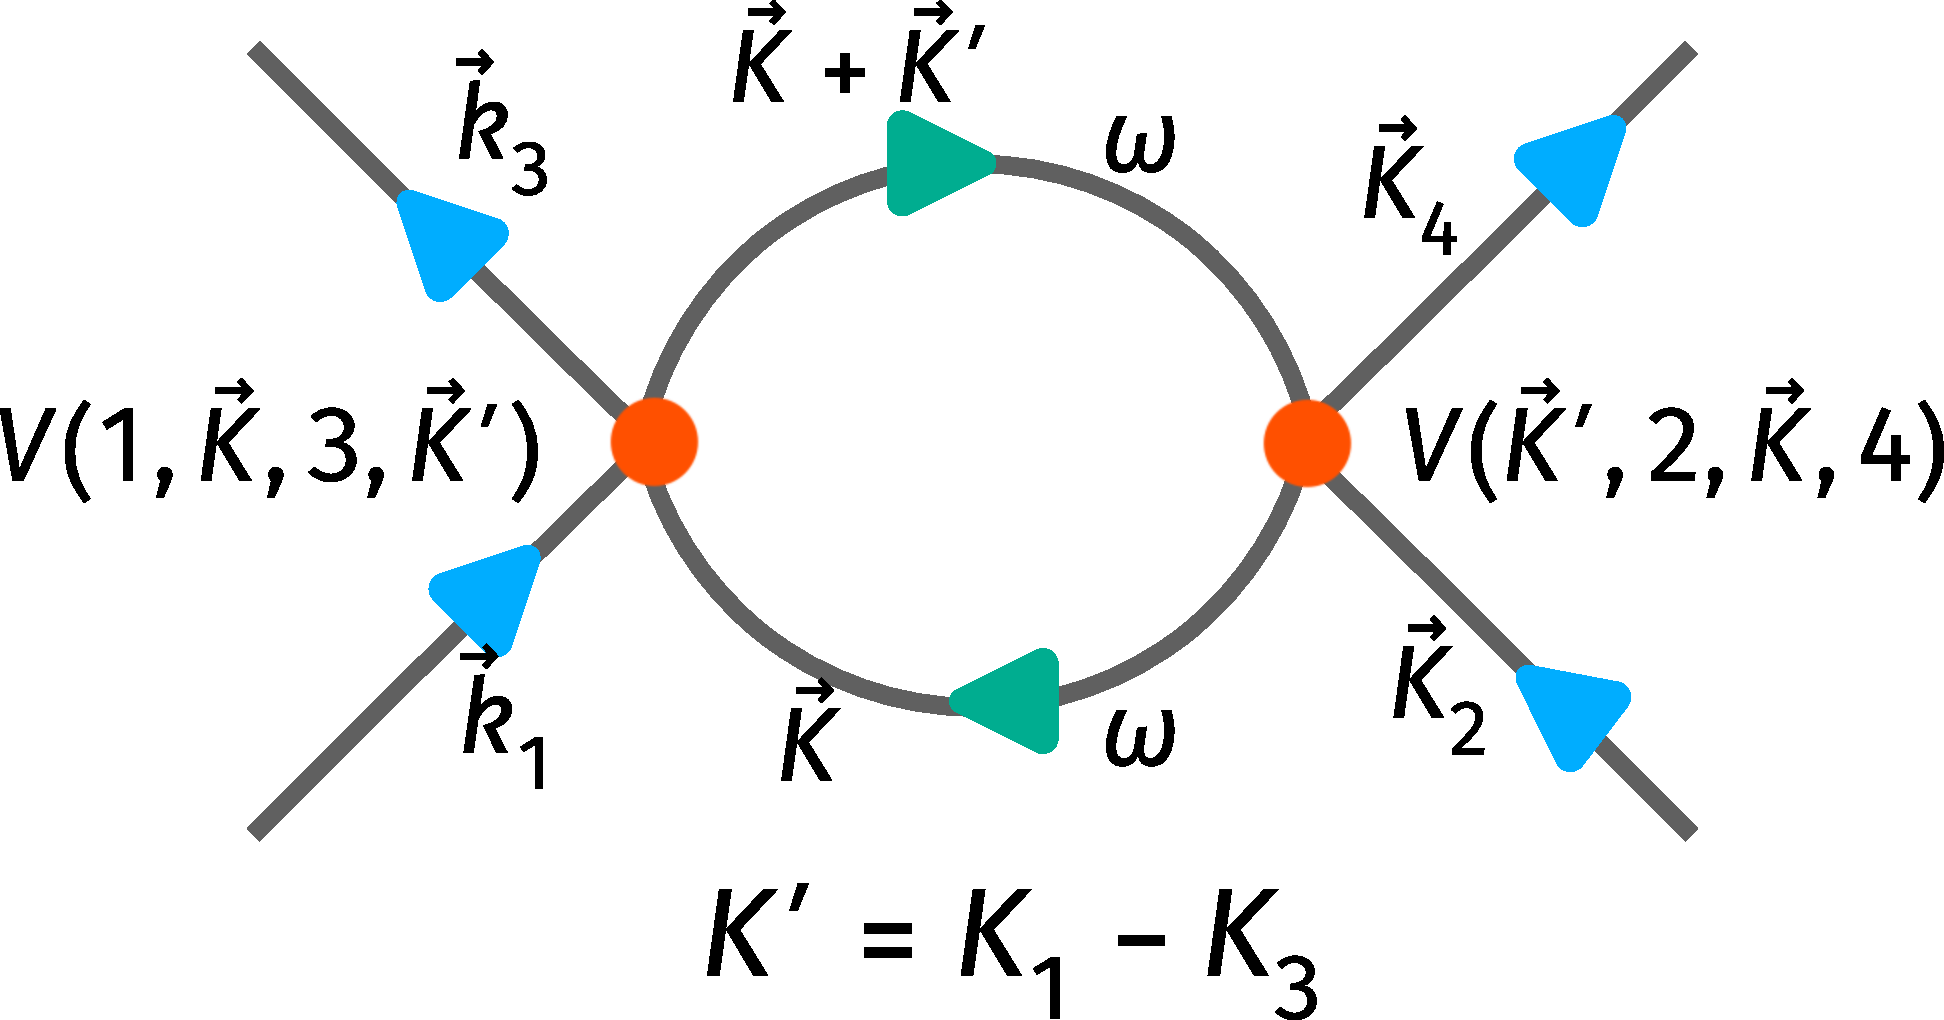
\includegraphics[width=0.5\textwidth]{./figures/term3.pdf}
\caption{ZS diagram for quartic interaction. \(K_1\) and \(K_3\) scatter into \(K_3\) and \(K_4\) respectively, through the exchange of virtual particles of momenta \(K + K_1 - K_3\) and \(K\).}
\label{loop11}
\end{figure}
The contribution to the action coming from this diagram is
\begin{equation}\begin{aligned}
	dV(1,2,3,4) = \int_{-\infty}^\infty d\omega  \int_0^{2\pi} d\theta \int_{\Lambda - d\Lambda}^\Lambda dK V(1,K,3,K+Q) V(K+Q, 2, K, 4) G_0(\omega, K)\\
	G_0(\omega, K+Q)
\end{aligned}\end{equation}
\(K\) and \(K+Q\) are the loop momenta, \(Q\) being the transferred momentum. \(Q\) is \(K_1 - K_3\) via momentum conservation at either vertex. The \(\theta\) being integrated over refers to the direction of the loop momenta. Both the \(\theta\) and \(K\) integrals are constrained such that both of the loop momenta lie within the annulus. \(G_0(\omega,K)\) is the non-interacting Greens function at frequency \(\omega\) and momentum \(K\):
\begin{equation}\begin{aligned}
	G_0(\omega,K) = \frac{1}{i\omega - \xi(K)}
\end{aligned}\end{equation}
\subsubsection{Contribution to \(V_1\) from ZS diagram}
Consider first the function \(V_1\), for which \(K_1=K_3\). The momentum transfer \(Q\) will be zero, and \(\theta\) can take any value from \(0\) to \(2\pi\), because \(K\) being on the annulus guarantees that \(K+Q\) is also on the annulus. The contribution then becomes
\begin{equation}\begin{aligned}
	dV_1(1,2) = 2\pi \int_{-\infty}^\infty d\omega \int_{\Lambda - d\Lambda}^\Lambda dK V(1,K,1,K) V(K, 2, K, 2) \left(\frac{1}{i\omega - \xi(K)}\right)^2
\end{aligned}\end{equation}
Both the poles of the integrand lie in the same half of the complex point, and more specifically at the same point \(\omega = -i\xi(K)\). This integral will be zero, because the contour can be closed in the other half of the complex plane, the one that does not have the pole.
\subsubsection{Contribution to \(V_2\) from ZS diagram}\label{V2_ZS}
For \(V_2\), we have \(K_1 + K_2 = K_3 + K_4 = 0\) which means \(Q\) can be non-zero, because \(K_1\) and \(K_3\) are uncorrelated. Assuming \(K\) lies in the positive region \(\left[\Lambda - d\Lambda, \Lambda\right]\), \(K+Q\) must lie either in that region or the negative region \(\left[-\Lambda, -\Lambda + d\Lambda\right]\). The former choice corresponds to small momentum transfer \(Q \ll \Lambda\), and with that choice, the two poles will again be on the same half of the complex plane: \(\xi(K) \simeq \xi(K+Q)\). To get a non-zero contribution, \(K+Q\) must lie on the region opposite to \(K\), and this corresponds to a large momentum transfer \(|Q| \sim k_F\). The contribution can be written as
\begin{equation}\begin{aligned}
	dV_2(1,3) = \int d\theta \int_{d\Lambda} dK  ~V(1,K,3,K+Q) V(K+Q, -1, K, -3)\\
	\int_{-\infty}^\infty d\omega\frac{1}{i\omega - \xi(K)}\frac{1}{i\omega - \xi(K+Q)}
\end{aligned}\end{equation}
The variation in the momenta \(K\) and \(K+Q\) is now completely in the angle \(\theta\). The \(K-\)integral can be taken care of by replacing it with \(|d\Lambda|\), because that is the width of momentum we are integrating over, and the variation is now purely in the orientation. The \(\omega\)-integral can be evaluated by substituting \(\xi(K) = -\xi(K+Q) \sim \Lambda\). With these simplifications, we get
\begin{equation}\begin{aligned}
	dV_2(1,3) \sim \frac{|d\Lambda|}{\Lambda}\int d\theta V(1,K,3,K+Q) V(K+Q, -1, K, -3)
\end{aligned}\end{equation}
The \(\theta-\)integral has to enforce two constraints: firstly, \(K+Q\) and \(K\) must lie on opposite annulus so as to create poles on opposite halves, and secondly, \(Q\) has to be of the order of \(k_F\) to give a non-zero integral. To find the range of \(\theta\) that satisfies these two constraints, let us imagine two separate constructions of the Fermi volume surrounded by the annuli of width \(d\Lambda\). The first construction is for \(K\) while the second one is for \(K+Q\). Without any constraint, both \(K\) and \(K+Q\) can take any orientation on the construction, and the distance between the centers of the two construction when the tips of \(K\) and \(K+Q\) overlap  then determine the transferred momentum \(Q\). This is shown in fig.~\ref{overlap}.
\begin{figure}[!htpb]
	\centering
	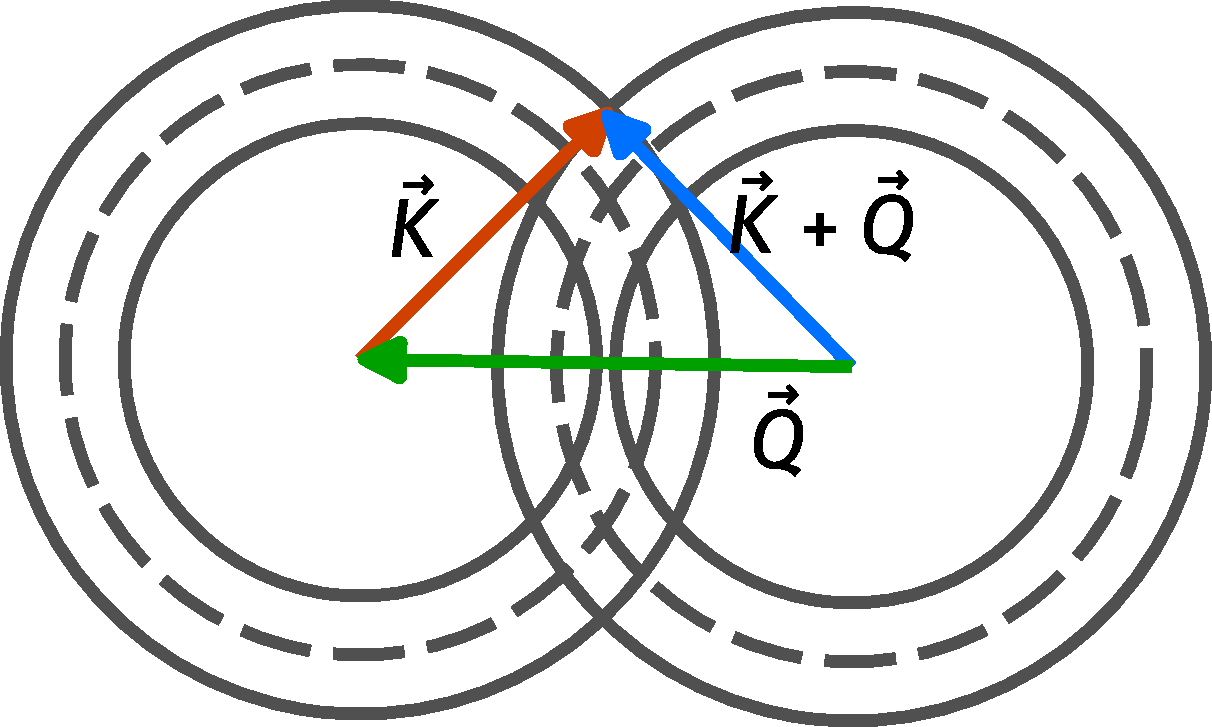
\includegraphics[width=0.4\textwidth]{./figures/overlap.pdf}
	\caption{Constructions for the two momenta \(K\) and \(K+Q\). The middle thin circle is the Fermi circle, while the thicker circles represent the annuli of width \(d\Lambda\). The heads of \(K\) and \(K+Q\) have been brought to the same point, the distance between the two centers gives the exchange momentum \(Q\). Rotating \(K+Q\) or \(K\) will require us to move the spheres either towards or apart from each other, leading to change in \(Q\).}
	\label{overlap}
\end{figure}

Varying the orientation of \(K+Q\) then leads to various distances between the centers of the two constructions, and hence to various values of \(Q\). In our case, since \(Q \sim k_F\), we need a specific distance between the constructions, and hence a specific set of orientations of \(K\) and \(K+Q\). These eight orientations are shown in fig.~\ref{overlap_survive}. 

\begin{figure}[!htpb]
	\centering
	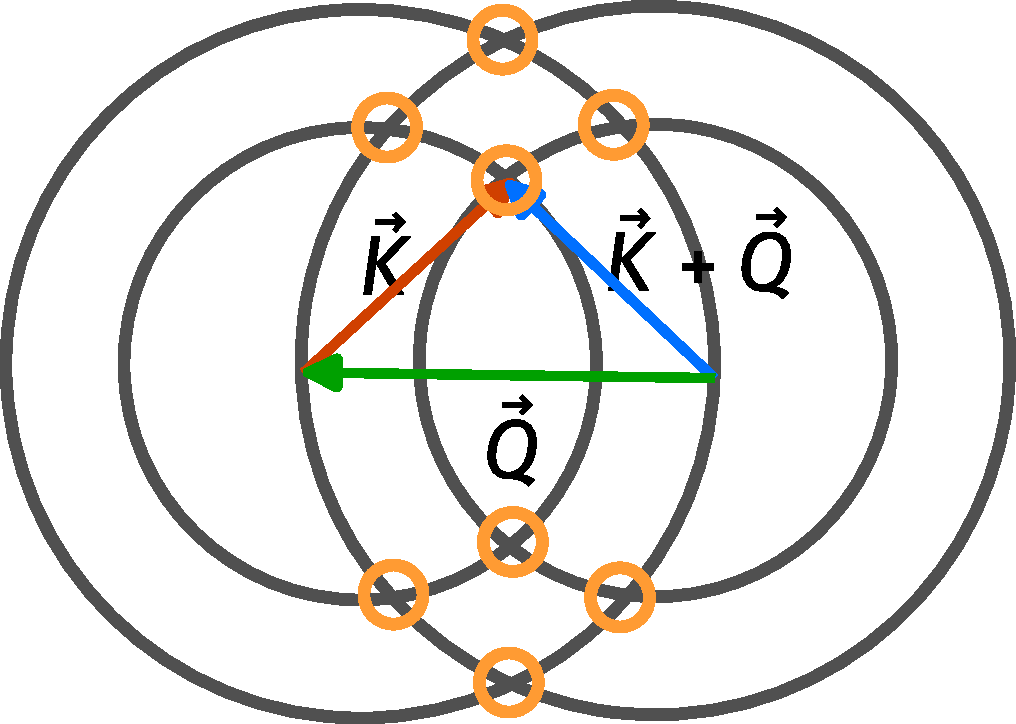
\includegraphics[width=0.35\textwidth]{./figures/overlap_survive.pdf}
	\caption{The same constructions, but the Fermi ring has not been drawn and the annuli have been made thicker for clarity.  The two centers have now been placed at a distance of \(k_F\) (which is just the radius of each sphere). The possible combinations of \(K\) and \(K+Q\) are now given by the intersections of the thick regions of each construction. There are eight such regions, marked by the yellow circles.}
	\label{overlap_survive}
\end{figure}

Each intersection region enclosed by the yellow rings subtends an angle of \(\frac{|d\Lambda|}{k_F}\), so the \(\theta\) integration is of the same order. The total integral is therefore of the order of
\begin{equation}\begin{aligned}
	dV_2(1,-1,3,-3) \sim \frac{|d\Lambda|}{\Lambda}\frac{|d\Lambda|}{k_F} V(1,K,3,K+Q) V(K+Q, -1, K, -3)
\end{aligned}\end{equation}
The RG equation takes the form
\begin{equation}\begin{aligned}
	\frac{d V_2}{dt} = \frac{d\Lambda}{k_F} V(1,K,3,K+Q) V(K+Q, -1, K, -3) \to 0
\end{aligned}\end{equation}
where \(dt = \frac{|d\Lambda|}{\Lambda}\). Since the RHS is infinitesimal, this contribution goes to zero in the continuum limit.
\subsection{ZS\(^\prime\) diagram}
The \(ZS^\prime\) diagram is the same as the \(ZS\) diagram, except for the fact that the labels \(3\) and \(4\) have to be interchanged. This interchange leads to a minus sign in the expression of the contribution of this diagram:
\begin{equation}\begin{aligned}
	dV(1,2,3,4) = -\int_{-\infty}^\infty d\omega  \int_0^{2\pi} d\theta \int_{d\Lambda}dK V(1,K,4,K+Q) V(K+Q, 2, K, 3) G_0(\omega, K)G_0(\omega, K+Q)
\end{aligned}\end{equation}
where the transferred momentum is now \(Q=K_1 - K_4\). For either the \(V_1\) channel or the \(V_2\) channel, \(Q\) need not be zero, because none of the channels correlate \(K_1\) with \(K_4\). This diagram is therefore similar to the \(V_2\) contribution to the \(ZS\)-diagram described in \ref{V2_ZS}, and it will go to zero for the same reason. We move on to the final diagram.
\subsection{BCS diagram}
\begin{minipage}{0.55\textwidth}
The final 1-loop diagram for the quartic interaction is shown in fig.~\ref{bcs_diagram}. At the bottom vertex, the incoming particles scatter into two virtual particles. Since the incoming particles are at zero frequency, the virtual particles have equal and opposite frequencies \(\pm \omega\). The momenta are decide by momentum conservation; the virtual momenta have to add up to \(K_1 + K_2\). For the \(V_1\) channel, the momentum transfer is again of order \(k_F\) and the angular integration is of order \(\frac{d\Lambda}{k_F}\), making the contribution infinitesimal as in the previous few cases. For the \(V_2\) channel, however, we have \(K_1 + K_2 = 0\), which means that the loop momenta are \(\pm K\), and for any value of \(\theta\), the poles will be on opposite halves. This means there will not by any suppression of the \(\theta\) integral.
\end{minipage}
\hspace*{\fill}
\begin{minipage}{0.4\textwidth}
	\centering
	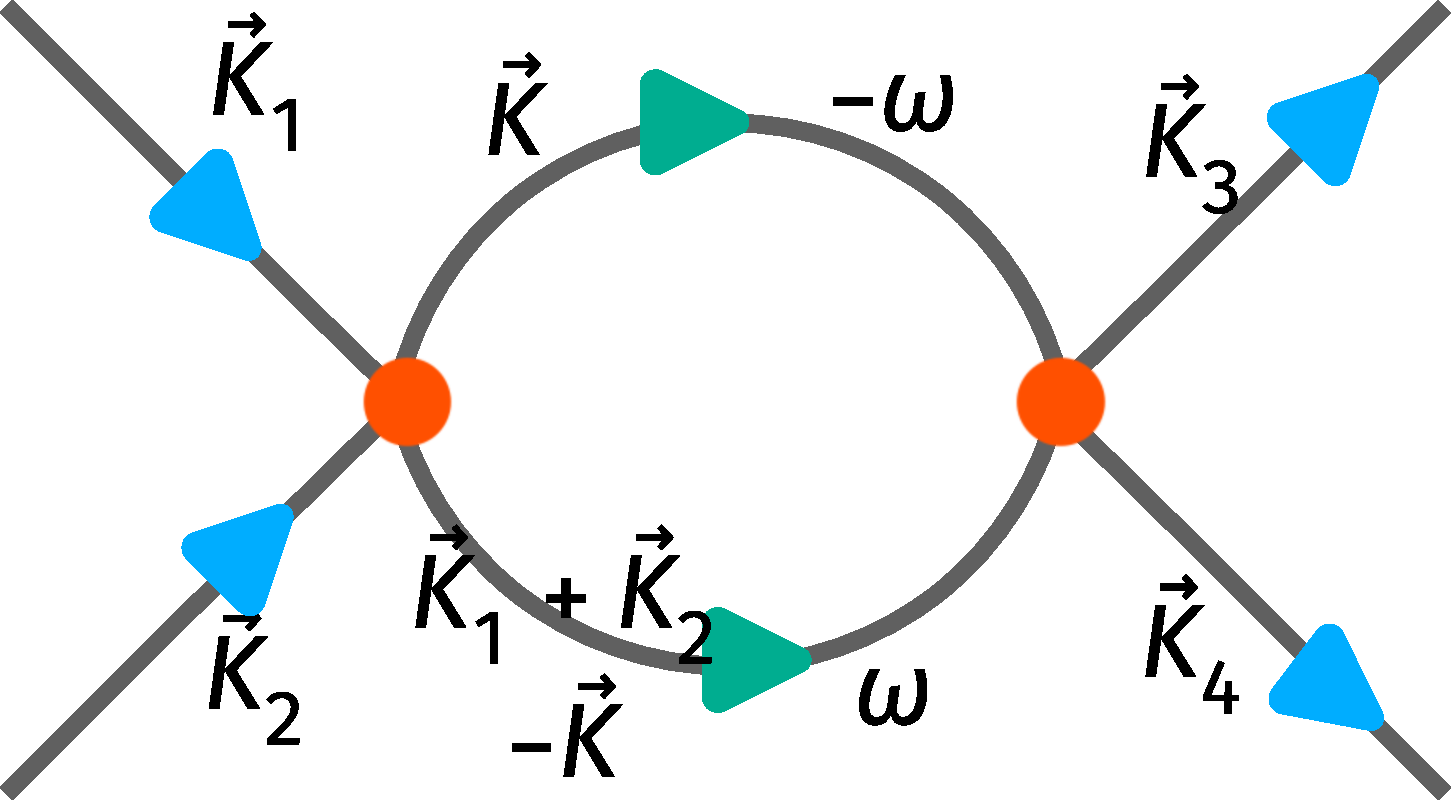
\includegraphics[width=0.8\textwidth]{./figures/term6.pdf}
	\captionof{figure}{BCS diagram.}
	\label{bcs_diagram}
\end{minipage}
\\\\
The contribution from this diagram for the \(V_2\) channel is
\begin{equation}\begin{aligned}
	dV_2(1,3) = -\frac{1}{2}\int_{-\infty}^\infty d\omega  \int_0^{2\pi} d\theta \int_{d\Lambda}dK V_2(1,K) V_2(K, 3) G_0(\omega, K)G_0(\omega, -K)
\end{aligned}\end{equation}
The minus sign comes from the fact that we need an odd number of Fermionic flips on the ZS diagram in order to achieve the BCS diagram. The factor of half arises from the fact that since \(K\) is being integrated over all values, each pair \(K, -K\) will be counted twice.The \(K-\)integral again gives a contribution of \(d\Lambda\), and the \(\omega-\)integration gives \(\frac{1}{\Lambda}\):
\begin{equation}\begin{aligned}
	dV_2(\theta_1 - \theta_3) = -\frac{|d\Lambda|}{2\Lambda}  \int_0^{2\pi} d\theta~ V_2(\theta_1 - \theta) V_2(\theta - \theta_3)
\end{aligned}\end{equation}
To solve this equation, note that since \(V_2\) depends only on the angular variable \(\theta_1 - \theta_3\), it can be expanded in a series of \(e^{im\theta}\), because the exponentials form a complete set:
\begin{equation}\begin{aligned}
	V_2(\theta_1 - \theta_3) = \sum_m v_m e^{im\left(\theta_1 - \theta_3\right)}
\end{aligned}\end{equation}
If we similarly expand the other \(V_2\) and substitute them in the coupling equation, we get
\begin{equation}\begin{aligned}
	\sum_m \frac{\mathrm{d}v_m}{\mathrm{d}t} e^{im\left(\theta_1 - \theta_3\right)} &= -\frac{1}{2}\int_0^{2\pi} d\theta \sum_{m_1,m_3}v_{m_1}v_{m_3}e^{i\left(m_1\theta_1 - m_3\theta_3\right)}e^{i\theta\left(m_3 - m_1\right)}\\
											   &=-\frac{1}{2}\sum_{m_1,m_3}v_{m_1}v_{m_3}e^{i\left(m_1\theta_1 - m_3\theta_3\right)}2\pi \delta\left(m_3 - m_1\right)\\
											   &=-\pi\sum_{m}v_m^2e^{im\left(\theta_1 - \theta_3\right)}\\
\end{aligned}\end{equation}
Since the \(\exp\left\{im\left(\theta_1 - \theta_3\right)\right\}\) form a linearly independent set, we can compare the coefficients directly and write down
\begin{equation}\begin{aligned}
\label{rgeq}
\frac{\mathrm{d}v_m}{\mathrm{d}t} &= -\pi v^2_{m} \implies v_m(t) = \frac{1}{v_m^{-1}(t_0) + \pi \left( t - t_0 \right) }
\end{aligned}\end{equation}
The RG equation \(\frac{\mathrm{d}v_m}{\mathrm{d}t} = -\pi v^2_{m}\) shows that as we increase \(t\), \(v_m\) always decreases, which means that a positive coupling will renormalize to 0 (irrelevant) while a negative coupling will renormalize to large negative values (relevant). The former corresponds to a Fermi liquid. The latter is the BCS instability. We can get an estimate of the BCS energy scale by noting the value of \(t\) at which the coupling diverges:
\begin{equation}\begin{aligned}
	v_m^{-1}(t_0) + \pi \left( t - t_0 \right)  = 0
\end{aligned}\end{equation}
Noting that \(t - t_0 = \ln \frac{\Lambda_0}{\Lambda}\), the equation gives
\begin{equation}\begin{aligned}
	\Lambda = \Lambda_0 \exp\left(\frac{\pi}{v_m(t_0)}\right)
\end{aligned}\end{equation}

\end{document}
